\chapter{Bayesian Methods}\label{uq:bayes}


This chapter covers specialized approaches for accelerating the 
Markov chain Monte Carlo (MCMC) sampling process using within
Bayesian inference.

\section{Fundamentals} \label{uq:bayes:basic}

Bayes Theorem~\cite{Jaynes}, shown in Eq.~\ref{eq:BayesThm}, is used
for performing inference.  In particular, we derive the plausible
parameter values based on the prior probability density and the data
$d$. A typical case involves the use of a conservative prior notion of
an uncertainty, which is then constrained to be consistent with the
observational data.  The result is the posterior parameter density of
the parameters $f_{\Theta |D}\left( {\theta |d} \right)$.
\begin{equation}
{f_{\Theta |D}}\left( {\theta |d} \right) = \frac{{{f_\Theta }\left( \theta  \right)\mathcal{L}\left( {\theta ;d} \right)}}{{{f_D}\left( d \right)}} \label{eq:BayesThm}
\end{equation}

The likelihood function is used to describe how well a model's
predictions are supported by the data.  
%The likelihood function can be written generally as:
%\begin{equation*}
%  \mathcal{L}\left( {\theta ;d} \right) = f\left( {q\left( \theta  \right) - d} \right)
%\end{equation*}
The specific likelihood function currently used in Dakota is a Gaussian
likelihood. This means that we assume the difference between the model quantity of interest
(e.g. result from a computer simulation) and the experimental observations are Gaussian:
\begin{equation}
d_i = q_i(\theta) + \epsilon_i, \label{eq:model}
\end{equation}
where $\theta$ are the parameters of a model quantity of interest $q$ and
$\epsilon_i$ is a random variable that can encompass both measurement
errors on $d_i$ and modeling errors associated with the simulation quantity of interest 
$q_i(\theta)$. %We further assume that all experiments and
%observations are independent.  
If we have $n$ observations, the probabilistic model defined by 
Eq.~(\ref{eq:model}) results in a likelihood function for $\theta$ 
%that is the product of $n$ normal probability density functions 
as shown in Eq.~\ref{eq:Likelihood}:
\begin{equation}
\mathcal{L}(\theta;d) \propto % = \frac{1}{(2\pi)^n |\boldsymbol{\Sigma}_d|} 
\exp \left(
-\frac{1}{2} \boldsymbol{r}^T \boldsymbol{\Sigma}_d^{-1} \boldsymbol{r} 
\right), \label{eq:Likelihood}
%\mathcal{L}({\theta};d) = \prod_{i=1}^n \frac{1}{\sigma \sqrt{2\pi}} \exp
%\left[ - \frac{\left(d_i-\mathcal{M}({\theta})\right)^2}{2\sigma^2} \right]
\end{equation}
where the residual vector $\boldsymbol{r}$ is defined from the
differences between the model predictions and the corresponding
observational data (i.e., $r_i = q_i(\theta) - d_i$ for $i = 1,\dots,n$),
$\boldsymbol{\Sigma}_d$ is the covariance matrix of the Gaussian data
uncertainties, and we omit the leading multivariate normal (MVN)
constant $1/\sqrt{(2\pi)^n |\boldsymbol{\Sigma}_d|}$ for 
simplicity\footnote{In practice, omitting this MVN constant can avoid 
  precision loss due to subtractive cancellation in log-likelihood 
  calculations; further, this shortcut will be canceled out by the 
  normalization factor in the denominator of Eq.~\ref{eq:BayesThm}.}. 
  % exception: calibrate sigma? (could rescale sigma after the fact)

The negative log-likelihood is known as the misfit function:
\begin{equation}
M(\theta;d) = \frac{1}{2} \boldsymbol{r}^T \boldsymbol{\Sigma}_d^{-1} 
\boldsymbol{r} % + C
\label{eq:misfit}
\end{equation}
It is evident that dropping $\boldsymbol{\Sigma}_d$ from this
expression (or equivalently, taking it to be the identity) results in
the ordinary least squares (OLS) approach commonly used in
deterministic calibration.  Minimizing the misfit function is
equivalent to maximizing the likelihood function and results in a
solution known as the maximum likelihood estimate (MLE), which will be
the same as the OLS estimate when the residuals have no relative
weighting (any multiple of identity in the data covariance matrix).

When incorporating the prior density, the maximum {\it a posteriori}
probability (MAP) point is the solution that maximizes the posterior
probability in Eq.~\ref{eq:BayesThm}.  This point will differ
from the MLE for cases of non-uniform prior probability.

%\begin{equation}
%p(\mathbf{d}|\xi) \;=\; \text{exp}\left[-\frac{1}{2}(f(\xi)-\mathbf{d})^T\boldsymbol{\Sigma}_d^{-1}(f(\xi)-\mathbf{d})\right]
%\end{equation}
%\begin{equation}
%-\text{log}\left[p(\mathbf{d}|\xi)\right] \;=\; \frac{1}{2}(f(\xi)-\mathbf{d})^T\boldsymbol{\Sigma}_d^{-1}(f(\xi)-\mathbf{d}) \;=\; M(\xi)
%\end{equation}

\section{Proposal Densities} \label{uq:bayes:prop}

When derivatives of $q(\theta)$ are readily available (e.g.,
from adjoint-capable simulations or from emulator models such as
polynomial chaos, stochastic collocation, or Gaussian processes), we
can form derivatives of the misfit function as
\begin{eqnarray}
\nabla_\theta M(\theta) &=& \nabla_\theta \boldsymbol{q}(\theta)^T\,\boldsymbol{\Sigma}_d^{-1}\,\boldsymbol{r} \label{eq:grad_misfit} \\
\nabla^2_\theta M(\theta) &=& \nabla_\theta \boldsymbol{q}(\theta)^T\,\boldsymbol{\Sigma}_d^{-1}\,\nabla_\theta \boldsymbol{q}(\theta) + \nabla^2_\theta \boldsymbol{q}(\theta) \cdot \left[\boldsymbol{\Sigma}_d^{-1}\,\boldsymbol{r}\right] \label{eq:hess_misfit}
\end{eqnarray}
Neglecting the second term in Eq.~\ref{eq:hess_misfit} (a
three-dimensional Hessian tensor dotted with the residual vector)
results in the Gauss-Newton approximation to the misfit Hessian:
\begin{equation}
\nabla^2_\theta M(\theta) \approx \nabla_\theta \boldsymbol{q}(\theta)^T\,\boldsymbol{\Sigma}_d^{-1}\,\nabla_\theta \boldsymbol{q}(\theta) \label{eq:hess_misfit_gn}
\end{equation}
This approximation requires only gradients of the residuals, enabling
its use in cases where models or model emulators only provide
first-order derivative information.  Since the second term in
Eq.~\ref{eq:hess_misfit} includes the residual vector, it becomes less
important as the residuals are driven toward zero.  This makes the
Gauss-Newton approximation a good approximation for solutions with
small residuals.

To form the MVN proposal density for the MCMC process, we define the
proposal covariance to be the inverse of the misfit Hessian.  Since
the full Hessian may be indefinite while the Gauss-Newton
approximation is at least positive semi-definite, we may first attempt
to invert the full Hessian, followed by recourse when necessary to
inverting the Gauss-Newton approximate Hessian.

\section{Rosenbrock Example} \label{uq:bayes:ex}

Defining two residuals as:
\begin{eqnarray}
r_1 &=& 10 (\theta_2 - \theta_1^2) \label{eq:rosen_r1} \\
r_2 &=& 1 - \theta_1 \label{eq:rosen_r2}
\end{eqnarray}
with $\boldsymbol{d} = \boldsymbol{0}$ and $\boldsymbol{\Sigma}_d =
\text{diag}(\boldsymbol{.5})$, it is evident from Eq.~\ref{eq:misfit}
that $M(\theta;d)$ is exactly the Rosenbrock function\footnote{The
  two-dimensional Rosenbrock test function is defined as $100 (x_2 -
  x_1^2)^2 + (1 - x_1)^2$} with its well-known banana-shaped contours.

Assuming a uniform prior on $[-2,2]$,
Figure~\ref{fig:rosen_prop_covar} shows the effect of different
proposal covariance options, with the default prior covariance in
Figure~\ref{fig:rosen_prop_covar}(a) and the misfit Hessian-based
proposal covariance in Figure~\ref{fig:rosen_prop_covar}(b).
\begin{figure}[htbp]
  \begin{subfigmatrix}{2}
  \subfigure[Proposal covariance defined from uniform prior.]{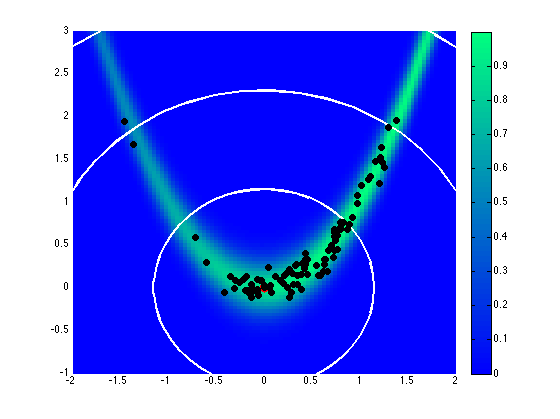
\includegraphics{images/rosen_00_prior}}
  \subfigure[Proposal covariance defined from misfit Hessian.]{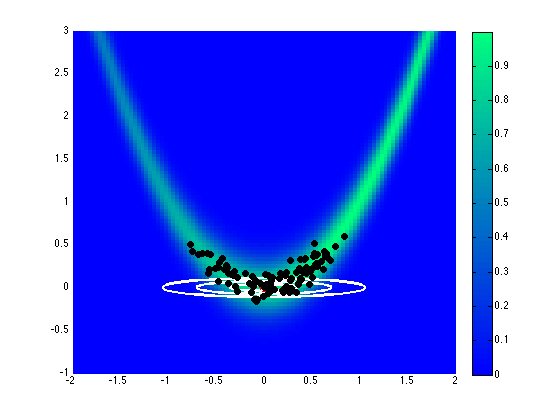
\includegraphics{images/rosen_00_pce_hessian}}
  \end{subfigmatrix}
  \caption{Depiction of proposal covariance at (0,0) with contours at one/two/three standard deviations.  2000 MCMC samples are performed and every 20th sample is plotted.}
\label{fig:rosen_prop_covar}
\end{figure}
Rejection rates for 2000 MCMC samples were 73.4\% for the former and
25.6\% for the latter.  Reducing the number of MCMC samples to 40, for
purposes of assessing locality, results in a similar 72.5\% rejection
rate for prior-based proposal covariance and a reduced 17.5\% rate for
misfit Hessian-based proposal covariance.  The prior-based proposal
covariance only provides a global scaling and omits information on the
structure of the likelihood; as a result, the rejection rates are
relatively high for this problem and are not a strong function of
location or chain length.  The misfit Hessian-based proposal
covariance, on the other hand, provides accurate local information on
the structure of the likelihood, resulting in low rejection rates for
samples in the vicinity of this Hessian update.  Once the chain moves
away from this vicinity, however, the misfit Hessian-based approach
may become inaccurate and actually impede progress. This implies the
need to regularly update the misfit Hessian-based proposal covariance
to sustain these MCMC improvements.

In Figure~\ref{fig:rosen_restart}, we show a result for a total of
2000 MCMC samples initiated from $(-1,1)$, where we restart the chain
with an updated misfit Hessian-based proposal covariance every 40
samples (Dakota specification: \texttt{proposal\_updates = 50}).  This
case uses a standard normal prior, resulting in differences in the MLE
and MAP estimates, as shown in Figure~\ref{fig:rosen_restart}(a).
Figure~\ref{fig:rosen_restart}(b) shows the history of rejection rates
for each of the 50 chains compared to the rejection rate for a single
2000-sample chain using prior-based proposal covariance.
\begin{figure}[htbp]
  \begin{subfigmatrix}{2}
  \subfigure[Restarted chain.]{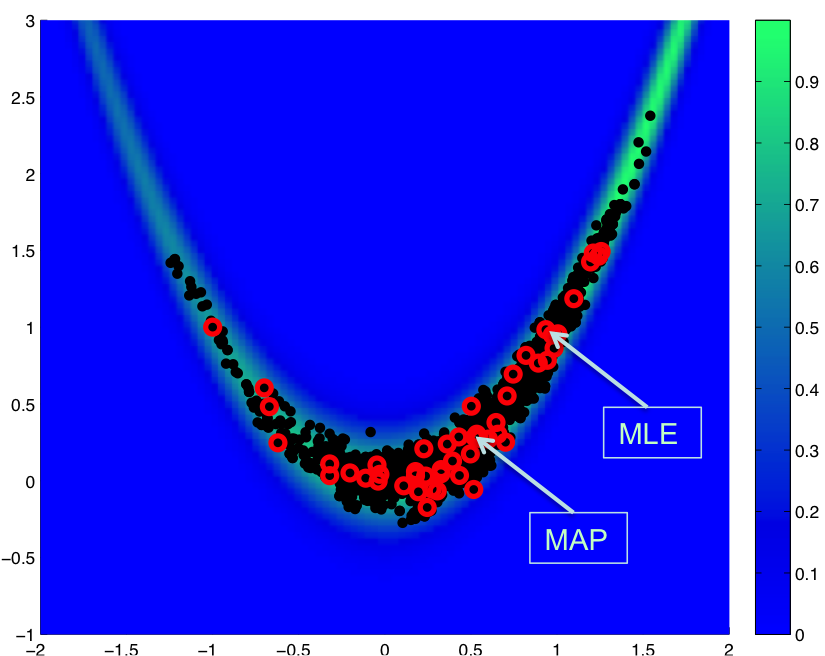
\includegraphics{images/rosen_restart_mle_map}}
  \subfigure[Rejection rates.]{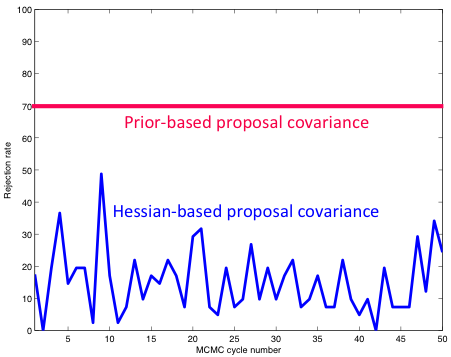
\includegraphics{images/rosen_restart_reject}}
  \end{subfigmatrix}
  \caption{MCMC chain with 2000 total samples, 50 proposal updates using the inverse of the misfit Hessian, and standard normal prior.}
\label{fig:rosen_restart}
\end{figure}
